\documentclass{article}\usepackage{amsmath,amssymb,amsthm,tikz,tkz-graph,color,chngpage,soul,hyperref,csquotes,graphicx,floatrow}\newcommand*{\QEDB}{\hfill\ensuremath{\square}}\newtheorem*{prop}{Proposition}\renewcommand{\theenumi}{\alph{enumi}}\usepackage[shortlabels]{enumitem}\usepackage[nobreak=true]{mdframed}\usetikzlibrary{matrix,calc}\MakeOuterQuote{"}\usepackage[margin=0.75in]{geometry} \newtheorem{theorem}{Theorem}
\newcommand{\dincludegraphics}[1]{\includegraphics[width=0.5\textwidth]{#1}}
\newcommand{\tincludegraphics}[1]{\includegraphics[width=0.33\textwidth]{#1}}

\title{EE16A - Lecture 15 Notes}
\author{Name: Felix Su$\quad$SID: 25794773}
\date{Spring 2016$\quad$GSI: Ena Hariyoshi}
\begin{document}
\maketitle

%%%% Topic %%%%
\subsection*{Scaling OpAmps}
%%%% Notes %%%%
\begin{center}\dincludegraphics{scaleop}\dincludegraphics{opvdac}\end{center}
\begin{itemize}
    \item Example at 46:53
    \item DAC: $V_{max}  = 3.3V$, $V_{min}= 0$
    \item Speakers can be modeled with an $8\Omega$ resistor to ground
    \item Need OpAmp to scale $V_{DAC}$ to the range of the speaker without creating a blocking pattern (shown above)
\end{itemize}
%%%% Topic %%%%
\subsection*{Negative Feedback Loop}
%%%% Notes %%%%
\begin{center}\dincludegraphics{nfl}\end{center}
\begin{itemize}
    \item Compare input against scaled feedback (from output)
    \item Feed result into a linear gain (A) to produce the output
    \item Send output into scaled feedback loop to compare against input
    \item If feedback $>$ input, error is negative, output is pushed down, which causes the feedback to go down... etc.
    \item If feedback $<$ input, error is positive, output is pushed up, which causes the feedback to go up... etc.
    \item Big Picture: Feedback will approach the input
\end{itemize}
%%%% Topic %%%%
\subsection*{Golden Rules}
%%%% Notes %%%%
\begin{center}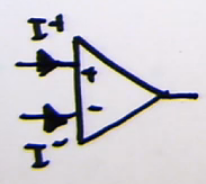
\includegraphics{opcurr}\end{center}
\begin{mdframed}
\begin{enumerate}[1.]
    \item $I^+ = I^- = 0$ (always true for ideal op amps)
    \item $V^+ = V^-$ (only true with negative feedback)
\end{enumerate}
\end{mdframed}
%%%% Topic %%%%
\subsection*{OpAmp Negative Feedback Loop Analysis}
%%%% Notes %%%%
\begin{center}\dincludegraphics{opnfl}\dincludegraphics{opnflkvl}\end{center}
\begin{itemize}
    \item Input voltage $V_{in}$ connected to OpAmp, with $V_{out}$
    \item Negative Feedback loop with $R_1$ connected to ground through parallel $R_2$ in and $V_{fb}$ between $V_{out}$ and $V^-$
    \item Because $V^-$ is an open circuit: $I_1 = I_2$
    \item GR 1. $I^+ = I^- = 0$ : KCL at node between $R_1$, $R_2$: $I_1 = I_2$ (because $I^- = 0$)
    \item GR 2. $V^+ = V^-$ : $V_{in} = V_{fb}$
    \item Ohm's Law on $R_2$ because $V_2 = V_{fb}$: $I_2 = \frac{V_{fb}}{R_2} = \frac{V_{in}}{R_2}= I_1$
    \item KVL of path from ground to $V_{out}$ through $R_1$ : $V_{out} = V_{fb}+I_1R_1 = V_{in}+\frac{V_{in}R_1}{R_2} = V_{in}(1+\frac{R_1}{R_2})$
\end{itemize}
\begin{mdframed}
\textbf{OpAmp Negative Feedback Loop Equations}
\begin{equation}I^+ = I^- = 0\end{equation}
\begin{equation}V^+ = V^-\end{equation}
\begin{equation}V_{out} = V_{in}(1+\frac{R_1}{R_2})\end{equation}
\end{mdframed}
\end{document}

